% Following magic comments allow for compilation of root file
% !TEX root = ../../../../temp_manuscript.tex

\chapter[Predicting the \acl{1p19qstat} of presumed low-grade glioma with an externally validated machine learning algorithm][SVM for 1p/19q prediction of LGG]{Predicting the \acl{1p19qstat} of presumed low-grade glioma with an externally validated machine learning algorithm}\label{chap:LGG1p19q}


\begin{ChapterAbstract}
    \textbf{Purpose:} Patients with \acl{1p19qcodel} \cgls{LGG} have longer overall survival and better treatment response than patients with \acl{1p19qint} \glspl{tumor}.
    Therefore, it is relevant to know the \acl{1p19qstat}.
    To investigate whether the \acl{1p19qstat} can be assessed prior to \gls{tumor} resection, we developed a machine learning algorithm to predict the \acl{1p19qstat} of presumed \cgls{LGG} based on preoperative \cgls{MRI}.

    \textbf{Experimental Design:} Preoperative brain \cgls{MR} images from 284 patients who had undergone biopsy or resection of presumed \cgls{LGG} were used to train a support vector machine algorithm.
    The algorithm was trained on the basis of features extracted from \cgls{T1C} and \cgls{T2} MR images and on patients' age and sex.
    The performance of the algorithm compared with tissue diagnosis was assessed on an external validation dataset of \cgls{MR} images from 129 patients with \cgls{LGG} from \cgls{TCIA}.
    Four clinical experts also predicted the \acl{1p19qstat} of the \cgls{TCIA} \cgls{MR} images.

    \textbf{Results:} The algorithm achieved an \cgls{AUC} of \num{0.72} in the external validation dataset.
    The algorithm had a higher predictive performance than the average of the neurosurgeons (\cgls{AUC} \num{0.52}) but lower than that of the neuroradiologists (\cgls{AUC} of \num{0.81}).
    There was a wide variability between clinical experts (\cgls{AUC} \numrange{0.45}{0.83}).

    \textbf{Conclusions:} Our results suggest that our algorithm can noninvasively predict the \acl{1p19qstat} of presumed \cgls{LGG} with a performance that on average outperformed the oncological neurosurgeons.
    Evaluation on an independent dataset indicates that our algorithm is robust and generalizable.

    \publishedas{vandervoort2019predictingcodeletion}
\end{ChapterAbstract}

\section{Introduction}

\cGls{LGG} is a primary brain \gls{tumor} that originates from glial cells.
The \cgls{WHO} 2016 criteria recognize three subtypes based on molecular and histologic features \autocite{louis20162016,van2017diffuse}:

\begin{enumerate}
\item Diffuse \cgls{IDH}-wildtype astrocytoma (\cgls{IDH}-wildtype, \acl{1p19qint})
\item Diffuse \cgls{IDH}-mutated astrocytoma (\cgls{IDH}-mutated, \acl{1p19qint})
\item Oligodendroglioma (\cgls{IDH}-mutated, \acl{1p19qcodel})
\end{enumerate}

Studies have shown that the distinction between these three categories is clinically relevant in terms of prognosis and management: in patients treated with optimal surgical resection, followed by radiotherapy with or without chemotherapy, median survival is longest of those with oligodendroglioma \autocite{cairncross2014benefit, dubbink2015molecular}.
In addition, studies have suggested that residual \gls{tumor} has a more negative impact on survival in \acl{1p19qint}, \cgls{IDH}-mutated astrocytomas than on \acl{1p19qcodel}, \cgls{IDH}-mutated oligodendrogliomas \autocite{wijnenga2017impact, clark2019extent}.
Therefore, the ability to predict the molecular subtypes of \cgls{LGG} at an early stage could provide better guidance of risk-benefit assessment and clinical decision making.

The recent shift from histopathology-based glioma classification to the molecular subtype-based \cgls{WHO} 2016 classification gave rise to neuro-oncologic radiogenomics research in which features seen on preoperative \cgls{MR} images are used to predict the genetic mutation status of glioma \autocite{smits2017imaging, gevaert2014glioblastoma, gutman2013mr}.
Features such as frontal \gls{tumor} localization, indistinct \gls{tumor} borders, heterogeneous \cgls{SI} on \cgls{T2} images, and both cortical and subcortical \gls{tumor} infiltration all suggest the presence of \acl{1p19qcotion} \autocite{smits2017imaging}.

One way of linking \cgls{MRI} features to \acl{1p19qstat} is through machine learning.
Although several studies have applied this method to datasets of patients with high-grade glioma, few studies have developed radiogenomics methodology in \cgls{LGG} \autocite{akkus2017predicting, li2017deep, chang2018deep, han2018non, lu2018machine, zhou2019machine}.
Of the ones that have, most have not used an independent test set and, therefore, it is difficult to estimate their actual performance in the real-world clinical setting \autocite{akkus2017predicting, li2017deep, chang2018deep, han2018non}.
\citeauthorref{lu2018machine} did use an independent test set, but this set contained a very limited number of \cgls{LGG} cases (N = 12).
\citeauthorref{zhou2019machine} used a test set consisting of \cgls{IDH}-mutated \cgls{LGG} and high-grade glioma to evaluate the \acl{1p19qcotion} prediction performance.
This is not an ideal test set as the \acl{1p19qstat} is not clinically relevant for high-grade glioma, and there is a selection bias of \cgls{IDH}-mutated \glspl{tumor} only.

The aim of this retrospective study was to develop a radiogenomics approach to predict the \acl{1p19qstat} of presumed \cgls{LGG} based on preoperative \cgls{MRI} features, with a machine learning algorithm that was validated on a large external dataset.

\section{Materials and Methods}
\subsection{\acrshort{EMC}/\acrshort{HMC} dataset}
\subsubsection{Study participants}

All patients aged 18 years or older newly diagnosed with presumed \cgls{LGG} and who underwent \gls{tumor} resection or biopsy between October 2002 and March 2017 at the \cgls{EMC} or the \cgls{HMC} were retrospectively included in the \cgls{EMC}/\cgls{HMC} dataset.
Patients were eligible if histopathologic diagnosis with molecular subclassification of the \acl{1p19qstat} and preoperative \cgls{T1C} and \cgls{T2} \cgls{MR} images were available.
The study was approved by the Medical Ethical Committee of Erasmus MC, who waived the need for written informed consent from the patients due to the retrospective nature of this study and the (emotional) burden that would result from contacting the patients or their relatives to obtain consent.
The study was performed in accordance with the 1964 Declaration of Helsinki and its later amendments or comparable ethical standards.

\subsubsection{Histopathologic diagnosis and molecular subclassification}

\Gls{tumor} samples were obtained from patients who underwent surgical resection or biopsy.
Histopathologic examination was performed by neuropathologists and further molecular subclassification of the \acl{1p19qstat} and/or \cgls{IDH} mutation status was performed as part of the diagnostic routine by molecular biologists using \cgls{FISH}, loss of heterozygosity analysis, and targeted next-generation sequencing panel using an Ion Torrent Personal Genome Machine (Life Technologies) or Ion S5XL or a \cgls{MLPA} assay (MRC-Holland) \autocite{dubbink2015molecular, dubbink2016diagnostic, riemenschneider2010molecular, bienkowski2018molecular}.
All \glspl{tumor} were subclassified on the basis of the \cgls{WHO} 2016 criteria.

\subsubsection{Imaging acquisition and postprocessing}

\cgls{MR} images were used that were acquired in the routine diagnostic process.
\cgls{T1C} and \cgls{T2} \cgls{MRI} sequences were used for the algorithm.
In many, but not all, patients, \cgls{FLAIR} imaging was also available.
As images were acquired at a number of sites, the imaging data were heterogeneous with a wide range of acquisition settings in voxel spacing, matrix size, echo time, repetition time, number of slices, slice thickness, and field strengths on scanners from three different manufacturers (General Electric, Philips, and Siemens).
An overview of the scanning settings is given in \cref{tab:LGG_1p19q_MRI_settings}.

All images were visually inspected by M. Smits and excluded if \cgls{MRI} artifacts were present.
Presumed \cgls{LGG} was defined as nonenhancing \gls{tumor}, as seen on the presurgical \cgls{T1C} \cgls{MR} image.
Therefore, all \cgls{T1C} images were reviewed and excluded if clear or solid enhancement was present.
When available, \cgls{T1} images were inspected for hemorrhage to prevent false-positive assessment of enhancement.
Although \glspl{tumor} with evident contrast enhancement were excluded, minimal enhancement was tolerated.
Minimal enhancement was defined as punctiform (\SI{<1}{\milli\meter} in diameter) or poorly defined faint enhancement, \citeauthorref[similar to][]{pallud2009prognostic}.

\Gls{tumor} segmentation was performed by two independent observers (F. Incekara and G. Kapas) using ITK-Snap \autocite{yushkevich2006user}.
Segmentation was done on \cgls{FLAIR} when available (\numbersamples{=119}), otherwise on the \cgls{T2} images (\numbersamples{=165}).
Because in our institution \cgls{LGG} segmentations are preferably performed on \cgls{FLAIR} images, we did not enforce the assessors to segment on \cgls{T2} images in order to stick to the real-world clinical practice.
The segmentations were then transformed to the \cgls{T2} images (in the case of \cgls{FLAIR} segmentation) and the \cgls{T1C} images, using the image registration software SimpleElastix \autocite{marstal2016simpleelastix}.
For all patients, brain masks were automatically constructed using FSL's BET tool with a fractional intensity threshold of \num{0.5} \autocite{smith2002fast}.
These brain masks were subsequently used to normalize the intensity of the \cgls{MR} images.
Details can be found in \cref{app:LGG_1p19q_algorithm}.

\subsection{\acrlong{TCIA} dataset}

Patients from \cgls{TCIA} \say{LGG-1p19qDeletion} dataset were screened for eligibility on the basis of previously described inclusion and exclusion criteria and used as the external validation dataset \autocite{akkus2017predicting, clark2013cancer, bradley2017radiology}.

This data collection is a publicly available dataset that consists of histopathologically proven \cgls{LGG} with coregistered \cgls{T1C} and \cgls{T2} preoperative \cgls{MRI} images as well as biopsy-proven \acl{1p19qstat}.
Molecular analysis of the \acl{1p19qstat} was performed with \cgls{FISH} for all \glspl{tumor}; \cgls{IDH} mutation status was not determined.
All \cgls{MRI} images were visually inspected by M. Smits as previously described.
An overview of the \cgls{MRI} settings is listed in \cref{tab:LGG_1p19q_MRI_settings}.
All \glspl{tumor} were semiautomatically segmented by M. Smits on the \cgls{T2} images using ITK-Snap.
Because the \cgls{T1C} and \cgls{T2} images were already coregistered in this study, the segmentation could be directly used for the \cgls{T1C} images without the need for registration.
Brain masks were made using FSL's BET tool, with the same settings as for the \cgls{EMC}/\cgls{HMC} dataset.

% \begin{table}
% \centering
% \setlength{\tabcolsep}{2.4pt}
% \begin{tabular}{L{2.5cm} R{1.1cm} R{1.1cm} R{1.1cm} R{1.1cm} R{1.1cm} R{1.1cm} R{1.1cm} R{1.1cm}}
%     \toprule
%     & \multicolumn{4}{c}{\thead{\acrshort{EMC}/\acrshort{HMC} (Training set)}} & \multicolumn{4}{c}{\thead{\acrshort{TCIA} (Validation set)}}\\
%     \cmidrule(l){2-5} \cmidrule(l){6-9}
%     \textbf{\acrshort{MRI} setting} & \multicolumn{2}{c}{\thead{\acrshort{T1C}}} & \multicolumn{2}{c}{\thead{\acrshort{T2}}} & \multicolumn{2}{c}{\thead{\acrshort{T1C}}} & \multicolumn{2}{c}{\thead{\acrshort{T2}}}\\
%     \midrule
%     \multicolumn{9}{l}{\textbf{Voxel spacing (mm)}}\\
%     & {\textit{Min}} & {\textit{Max}} & {\textit{Min}} & {\textit{Max}} & {\textit{Min}} & {\textit{Max}} & {\textit{Min}} & {\textit{Max}}\\
%     \cmidrule(l{15pt}){2-2} \cmidrule(l{15pt}){3-3} \cmidrule(l{15pt}){4-4} \cmidrule(l{15pt}){5-5} \cmidrule(l{15pt}){6-6} \cmidrule(l{15pt}){7-7} \cmidrule(l{15pt}){8-8} \cmidrule(l{15pt}){9-9}
%     \hspace{1em}Axial &\num{0.9}\hphantom{1} & \num{7.2} & \num{1.0} & \num{7.2} & \num{1.0} & \num{5.0} & \num{2.0} &\num{5.0}\\
%     \hspace{1em}Sagittal& \num{0.38} & \num{1.13} & \num{0.23} & \num{1.02} & \num{0.47} & \num{1.1} & \num{0.43} & \num{1.1}\\
%     \hspace{1em}Coronal & \num{0.38} & \num{1.13} & \num{0.23} & \num{1.02} & \num{0.47} & \num{1.1} &\num{0.43} &\num{1.1}\\
%     \addlinespace
%     \multicolumn{9}{l}{\textbf{Matrix size (number of voxels)}}\\
%     & {\textit{Min}} & {\textit{Max}} & {\textit{Min}} & {\textit{Max}} & {\textit{Min}} & {\textit{Max}} & {\textit{Min}} & {\textit{Max}}\\
%     \cmidrule(l{15pt}){2-2} \cmidrule(l{15pt}){3-3} \cmidrule(l{15pt}){4-4} \cmidrule(l{15pt}){5-5} \cmidrule(l{15pt}){6-6} \cmidrule(l{15pt}){7-7} \cmidrule(l{15pt}){8-8} \cmidrule(l{15pt}){9-9}
%     \hspace{1em}Axial&\num{19} & \num{248} & \num{19} & \num{304} & \num{20} & \num{196} & \num{20} & \num{84}\\
%     \hspace{1em}Sagittal& \num{256} & \num{1024} & \num{256} & \num{1024} & \num{256} & \num{512} & \num{256} & \num{512}\\
%     \hspace{1em}Coronal& \num{176} & \num{307} & \num{224} & \num{1024} & \num{256} & \num{512} & \num{256} & \num{512}\\
%     \addlinespace
%     \multicolumn{9}{l}{\textbf{Pulse sequence parameters (ms)}}\\
%     & {\textit{Min}} & {\textit{Max}} & {\textit{Min}} & {\textit{Max}} & {\textit{Min}} & {\textit{Max}} & {\textit{Min}} & {\textit{Max}}\\
%     \cmidrule(l{15pt}){2-2} \cmidrule(l{15pt}){3-3} \cmidrule(l{15pt}){4-4} \cmidrule(l{15pt}){5-5} \cmidrule(l{15pt}){6-6} \cmidrule(l{15pt}){7-7} \cmidrule(l{15pt}){8-8} \cmidrule(l{15pt}){9-9}
%     \hspace{1em}Echo time & \num{1.7} & \num{20} & \num{79.2} & \num{379} & \num{2.6} & \num{21} & \num{12.3} & \num{108.3}\\
%     \hspace{1em}Repetition time & \num{3.8} & \num{1940} & \num{2000} & \num{13468} & \num{8.2} & \num{983.3} & \num{2033.3} & \num{8116.6}\\
%     \addlinespace
%     \multicolumn{9}{l}{\textbf{Scanner settings}}\\
%     \multicolumn{2}{l}{\hspace{1em}Field strength (T)} & \multicolumn{2}{c}{\numlist{0.5;1.5;3.0}} & & & \multicolumn{2}{c}{\numlist{1.5;3.0}}\\
%     \hspace{1em}2D scans (\#)& \multicolumn{2}{c}{\num{147}} & \multicolumn{2}{c}{\num{264}} &\multicolumn{2}{c}{\num{33}} & \multicolumn{2}{c}{\num{129}}\\
%     \hspace{1em}3D scans (\#)& \multicolumn{2}{c}{\num{137}} & \multicolumn{2}{c}{\num{20}} &\multicolumn{2}{c}{\num{96}} & \multicolumn{2}{c}{\num{0}}\\
%     \bottomrule
% \end{tabular}
% \caption{Overview of the \acrshort{MRI} settings from the \acrshort{EMC}/\acrshort{HMC} and \acrshort{TCIA} datasets}\label{tab:LGG_1p19q_MRI_settings}
% \end{table}


\begin{table}
    \centering
    % \setlength{\tabcolsep}{2.4pt}
    \begin{tabular}{L{2.9cm} C{1.8cm} C{1.8cm} L{0.1cm} C{1.65cm} C{1.65cm}}
        \toprule
        & \multicolumn{2}{c}{\thead{\acrshort{EMC}/\acrshort{HMC}\\(Training set)}} && \multicolumn{2}{c}{\thead{\acrshort{TCIA}\\(Validation set)}}\\
        \midrule
        & \multicolumn{1}{c}{\thead{\acrshort{T1C}}} & \multicolumn{1}{c}{\thead{\acrshort{T2}}} && \multicolumn{1}{c}{\thead{\acrshort{T1C}}} & \multicolumn{1}{c}{\thead{\acrshort{T2}}}\\
        \cmidrule(lr){2-2} \cmidrule(lr){3-3} \cmidrule(lr){5-5} \cmidrule(lr){6-6}
        \\
        \multicolumn{5}{l}{\textbf{Voxel spacing (mm)}}\\
        \hspace{1em}Axial &0.9 -- 7.2& 1.0 -- 7.2&& \hphantom{0}1.0 -- 5.0& \hphantom{0}2.0 -- 5.0\\
        \hspace{1em}Sagittal &0.38 -- 1.13&0.23 -- 1.02  && 0.47 -- 1.1 & 0.43 -- 1.1\\
        \hspace{1em}Coronal & 0.38 -- 1.13& 0.23 -- 1.02 && 0.47 -- 1.1 & 0.43 -- 1.1\\
        \\
        % \addlinespace
        \multicolumn{5}{l}{\textbf{Matrix size (number of voxels)}}\\
        \hspace{1em}Axial & 19 -- 248 & 19 -- 304 && \hphantom{0}20 -- 196 & 20 -- 84\\
        \hspace{1em}Sagittal & 256 -- 1024 & 256 -- 1024 && 256 -- 512 & 256 -- 512\\
        \hspace{1em}Coronal & 176 -- 307\hphantom{0} & 224 -- 1024 && 256 -- 512 & 256 -- 512\\
        \\
        \multicolumn{5}{l}{\textbf{Pulse sequence parameters (ms)}}\\
        \hspace{1em}Echo time& 1.7 -- 20 & 79.2 -- 379\hphantom{00} && 2.6 -- 21\hphantom{0.} &12.3 -- 108.3\\
        \hspace{1em}Repetition time& \hphantom{00}3.8 -- 1940 & 2000 -- 13468 && \hphantom{0}8.2 -- 983.3 & 2033 -- 8116\\
        \\
        \multicolumn{5}{l}{\textbf{Scanner settings}}\\
        \hspace{1em}Field strength (T) & \multicolumn{2}{c}{0.5, 1.5, and 3.0} & & \multicolumn{2}{c}{1.5 and 3.0}\\
        \hspace{1em}2D scans (\#)& 147 & 264 &&33 & 129\\
        \hspace{1em}3D scans (\#)& 137 & 20 &&96 & 0\\
        \bottomrule
    \end{tabular}
    \caption{Overview of the \acrshort{MRI} settings from the \acrshort{EMC}/\acrshort{HMC} and \acrshort{TCIA} datasets}\label{tab:LGG_1p19q_MRI_settings}
    \end{table}


\subsection{Classification algorithm}

To predict the \acl{1p19qstat} of the \glspl{tumor} based on \cgls{MRI} features, the PREDICT toolbox was used.
This toolbox was used to extract a total of 78 image features (such as image intensity, \gls{tumor} texture, \gls{tumor} shape, and \gls{tumor} location) from the \cgls{T1C} and \cgls{T2} \cgls{MR} image.
These features, as well as the age and sex of the patient, were then used to train a \cgls{SVM}, resulting in a total of 80 features.
All parameter optimization and classifier training was performed on the \cgls{EMC}/\cgls{HMC} training set using 100 iterations of stratified random-split cross-validation, with \per{80} of the dataset used for training and \per{20} used for validation.
Once the algorithm was optimized, no more changes were made to the algorithm and it was then evaluated on the \cgls{TCIA} dataset.
To evaluate the algorithm, the accuracy, sensitivity (\acl{1p19qcotion} prediction), specificity (\acl{1p19qint} prediction), \cgls{AUC}, weighted F1 score, and precision were determined by comparing the predicted labels with the reference labels obtained from tissue diagnosis.
Full details of the algorithm can be found in the \cref{app:LGG_1p19q_algorithm}.
An overview of the classification algorithm is provided in \cref{fig:LGG_1p19q_radiomics_pipeline}.


\begin{figure}
    \centering
    \resizebox{\textwidth}{!}{
    \subimport{Figures/}{PREDICT_pipeline.pgf}
    }
    \caption{Overview of the radiomics pipeline}\label{fig:LGG_1p19q_radiomics_pipeline}
\end{figure}


To minimize the variance due to randomness in the algorithm training, an ensemble of five \cglspl{SVM}, which averages the predictions of the five independently trained models, was also constructed; the details can be found in \cref{app:LGG_1p19q_algorithm}.
One hundred different ensembles were constructed and were evaluated on the \cgls{TCIA} dataset using the evaluation metrics described previously.
Mean and standard deviation of the metrics over the 100 ensembles were computed.

To evaluate the contribution of the different features to the final prediction, a sensitivity analysis using polynomial chaos expansions was performed, resulting in Sobol indices for each feature \autocite{sudret2008global}.
The total Sobol index was used to determine the relative feature importance of the individual features.
The total Sobol index is a relative measure of the sensitivity of the algorithm to the input features.
The OpenPC toolbox was used to create the polynomial chaos expansions and to calculate the Sobol indices \autocite{perko2016fast, van2016robustness}.

We also determined which patients from the \cgls{TCIA} dataset were considered as representative examples for the \acl{1p19qcodel} and \acl{1p19qint} class by the algorithm.
This was achieved by counting the number of times the algorithm correctly predicted the class for a specific patient in the 100 ensembles that were constructed.

We also evaluated the performance of the algorithm when the \cgls{EMC}/\cgls{HMC} and \cgls{TCIA} dataset were mixed instead of used as a separate train and validation set to evaluate the effect of adding additional training data.
\subsection{Prediction of \acl{1p19qstat} by clinical experts}

To compare the results of the algorithm with expert performance, the \acl{1p19qstat} of the \cgls{TCIA} \glspl{tumor} was also predicted by two neuroradiologists and two neurosurgeons at the Erasmus MC Brain Tumor Centre.
They were presented with the \cgls{T1C} and \cgls{T2} images side by side for each patient as well as the sex and age to ensure that the algorithm and the raters had access to the same information.
For each \gls{tumor}, the raters were then asked to choose whether they thought it was \acl{1p19qcodel} or \acl{1p19qint} to provide a confidence score ranging from 1 to 5 (1 indicating very unsure and 5 indicating very sure).
This confidence score was then turned into a prediction \say{score} by dividing it by 5 and multiplying it by 1 if the predicted label was \acl{1p19qcodel} or by -1 if the predicted label was \acl{1p19qint}.
In this way, an \cgls{AUC} could be determined for the manual classification.
The accuracy, sensitivity, and specificity were determined in the same way as for the algorithm.

\subsection{Statistical analysis}

Statistical analyses to test differences between the two datasets were performed with SPSS \num{21.0} statistical software (IBM Corp.).
We tested whether the two datasets differed significantly from each other using the Mann-Whitney U test for continuous, nonnormally distributed variables (age and volume) and the $\chi^2$ test for all other categorical variables (sex, genetic analysis, presence of mild enhancement, \acl{1p19qstat}).
Predictive performances (mean and \per{95} \cgls{CI}) between the \cgls{EMC}/\cgls{HMC} training set and \cgls{TCIA} validation set were tested with the Welch t test.
Accuracy between the clinical experts and the algorithm was tested with the McNemar test.
A P value of \num{<0.05} was considered statistically significant.
The \per{95} \cglspl{CI} were calculated such that if the entire experiment of training on \cgls{EMC}/\cgls{HMC} and prediction on \cgls{TCIA} would be repeated in \per{95} of the repetitions, the result would lie within that interval.

\subsection{Data sharing}

The data used in this study are available on Mendeley Data (\url{http://doi.org/dj5k}).
The code for the construction and evaluation of the prediction algorithm is available on GitHub (\url{https://github.com/Svdvoort/PREDICT}).
The code used to construct the polynomial chaos expansions and calculate the Sobol indices is available on GitHub as well \hfill \break (\url{https://github.com/Svdvoort/OpenPC}).


\section{Results}

In the \cgls{EMC}/\cgls{HMC} dataset, 424 \cglspl{LGG} were identified and screened for eligibility.
Cases were excluded because of unknown \acl{1p19qstat} (\numbersamples{=22}), absence of \cgls{T1C} and/or \cgls{T2} \cgls{MRI} images (\numbersamples{=46}), enhancement (\numbersamples{=58}), and unacceptable image quality (\numbersamples{=14}), which resulted in 284 patients included for final analysis (flowchart, \cref{fig:LGG_1p19q_flowchart}).

\begin{figure}
\centering

\resizebox{0.8\textwidth}{!}{\subimport{Figures/}{inclusion_flowchart.pgf}}
\caption{Flow diagram of the inclusion procedure for both the \acrshort{EMC}/\acrshort{HMC} training dataset and \acrshort{TCIA} validation dataset}\label{fig:LGG_1p19q_flowchart}
\end{figure}


From the \cgls{TCIA} database, all 159 patients were screened for eligibility.
Patients were excluded because of enhancement (\numbersamples{=18}), signs of prior biopsy/surgical procedure (\numbersamples{=7}), no \cgls{T1C} imaging available (\numbersamples{=3}), and patients being younger than 18 years (\numbersamples{=2}), resulting in 129 patients included in the external validation dataset (flowchart, \cref{fig:LGG_1p19q_flowchart}).
An overview of the excluded patients from the \cgls{TCIA} database as well as the reason for exclusion is available in \cref{app:LGG_1p19q_exclusion}.

There was no significant difference between the \cgls{EMC}/\cgls{HMC} and \cgls{TCIA} datasets for median age (\num{43.0} years, \cgls{IQR}: \num{17.0}, vs.\ \num{39.0} years, \cgls{IQR}: \num{19.5}, respectively; \pvalue{ =0.11}) and sex distribution (\per{56.7} vs.\ \per{52.7} male, respectively; \pvalue{= 0.45}).
Median \gls{tumor} volume in the \cgls{EMC}/\cgls{HMC} dataset was significantly larger than in the \cgls{TCIA} dataset (median: \SI{47.80}{\centi\meter\cubed}, \cgls{IQR}: \num{58.65} vs.\ median \SI{35.70}{\centi\meter\cubed}, \cgls{IQR}: \num{49.10}, \pvalue{= 0.04}).
There were fewer \acl{1p19qcodel} \glspl{tumor} in the \cgls{EMC}/\cgls{HMC} compared with the \cgls{TCIA} dataset (\per{35.20} vs.\ \per{65.40}, \pvalue{< 0.0001}).
Patient and \gls{tumor} characteristics of both datasets are further presented in \cref{tab:LGG_1p19q_characteristics}.

\begin{table}[htbp]
    \sisetup{
    table-number-alignment = center,
    table-text-alignment = center,
    table-figures-integer = 1,
    table-figures-decimal = 4,
    }
\begin{tabular}{L{4.3cm} S[table-number-alignment=center-decimal-marker, table-format=3.0] S[table-number-alignment=center-decimal-marker, table-format=3.1] S[table-number-alignment=center-decimal-marker, table-format=3.0] S[table-number-alignment=center-decimal-marker, table-format=3.1] S[table-comparator = true]}
    \toprule
    & \multicolumn{2}{c}{\thead{\acrshort{EMC}/\acrshort{HMC}\\Training set\\(\numbersamples{=284})}} & \multicolumn{2}{c}{\thead{\acrshort{TCIA}\\Validation set\\(\numbersamples{=129})}} & {\thead{P-value}} \\
    \cmidrule(lr){2-3} \cmidrule(lr){4-5}
     &{N} &{\si{\percent}} &{N} &{\si{\percent}}\\
    \midrule

    \bfseries{Clinical}\\
    \hspace{1em}Age median [\acrshort{IQR}] (years) & \multicolumn{2}{c}{\IQR{43}{17}} & \multicolumn{2}{c}{\IQR{39}{19.5}} & 0.11\\
    \hspace{1em}Sex& & & & &0.45\\
    \hspace{2em}Male & 161 & 56.7 & 68 & 52.7\\
    \hspace{2em}Female & 123 & 43.3 & 61 & 47.3\\
\\
    \bfseries{Imaging}\\
    \hspace{1em}Volume median [\acrshort{IQR}] (\si{\centi\meter\cubed})& \multicolumn{2}{c}{\IQR{47.8}{58.7}} & \multicolumn{2}{c}{\IQR{35.7}{49.1}} & 0.04\\
    \hspace{1em}Mild enhancement & & & & &0.005\\
    \hspace{2em}Yes & 27 & 9.5 & 25 & 19.4\\
    \hspace{2em}No & 257 & 90.5 & 104 & 80.6\\
\\
    \multicolumn{2}{l}{\bfseries{Histopathology (\acrshort{WHO}, 2016)}} & & & & <0.0001\\
    \hspace{1em}Oligodendroglioma & 100 & 35.2 & 85 & 65.9\\
    \hspace{1em}Astrocytoma & 181 & 63.7 & 44 & 34.1\\
    \hspace{1em}Glioblastoma & 3 & 1.1 & 0 & 0.0\\
\\
    \bfseries{Genetic}\\
    \hspace{1em}\acl{1p19qcotion} & &  & &&<0.0001\\
    \hspace{2em}Yes & 100 & 35.2 & 85 & 65.9\\
    \hspace{2em}No & 184 & 64.8 & 44 & 34.1\\
    \hspace{1em}\acrshort{IDH} mutation & & & & & {\NA}\\
    \hspace{2em}Yes & 214 & 75.4 & 0 & 0.0\\
    \hspace{2em}No & 35 & 12.3 & 0 & 0.0\\
    \hspace{2em}Unknown & 35 & 12.3 & 129 & 100.0\\

    \hspace{1em}Method of analysis & & & &&<0.0001\\
    \hspace{2em}\acrshort{NGS} & 214 & 75.4 & 0 & 0.0 \\
    \hspace{2em}\acrshort{FISH} & 45 & 15.8 & 129 & 100.0\\
    \hspace{2em}\acrshort{MLPA} & 25 & 8.8 & 0 & 0.0\\
    \bottomrule
\end{tabular}
\caption{Patient and \gls{tumor} characteristics. Abbreviations: \acrcaption{IQR}, \acrcaption{NGS}, \acrcaption{FISH}, \acrcaption{MLPA}}\label{tab:LGG_1p19q_characteristics}
\end{table}

The predictive performance of the algorithm on the \cgls{EMC}/\cgls{HMC} training dataset, obtained from the cross validation, and the \cgls{TCIA} validation dataset is given in terms of accuracy, \cgls{AUC}, F1 score, precision, sensitivity, and specificity in \cref{tab:LGG_1p19q_svm_results}.
The accuracy, \cgls{AUC}, and sensitivity did not differ significantly between training and validation datasets (\pvalue{=0.886}, \pvalue{=0.746}, and \pvalue{=0.146}, respectively), whereas the specificity was significantly lower in the validation dataset (\pvalue{=0.038}).

\begin{table}[htbp]
    \sisetup{
    table-number-alignment = center,
    table-text-alignment = center,
    }
    \begin{tabular}{L{2cm} S[table-format=1.3] S[table-format=2.7] S[table-format=1.3]  S[table-format=2.7] S[table-format=1.3, table-comparator = true]}
        \toprule
        & \multicolumn{2}{c}{\thead{\acrshort{EMC}/\acrshort{HMC}\\Training set\\(\numbersamples{=284})}} & \multicolumn{2}{c}{\thead{\acrshort{TCIA}\\Validation set\\(\numbersamples{=129})}} \\
        \cmidrule(lr){2-3} \cmidrule(lr){4-5}
        & {Mean} & {\SI{95}{\percent} CI} & {Mean} & {\SI{95}{\percent} CI} & {P-value}\\
        \midrule
        Accuracy & 0.698 & \numrange{0.636}{0.760} & 0.693 & \numrange{0.657}{0.729} & 0.872\\
        \acrshort{AUC} & 0.755 & \numrange{0.694}{0.817} & 0.723 &\numrange{0.708}{0.737} & 0.313\\
        F1-score & 0.701 & \numrange{0.640}{0.761} & 0.697 & \numrange{0.661}{0.733} & 0.896\\
        Precision & 0.570 & \numrange{0.491}{0.649} & 0.787 & \numrange{0.754}{0.820} & <0.001\\
        Sensitivity & 0.657 & \numrange{0.562}{0.752} & 0.732 & \numrange{0.689}{0.775} & 0.123\\
        Specificity & 0.721 & \numrange{0.628}{0.813} & 0.717 & \numrange{0.544}{0.691} & 0.027\\
        \bottomrule
    \end{tabular}
    \caption{Predictive performances of the algorithm on the \acrshort{EMC}/\acrshort{HMC} training and \acrshort{TCIA} validation datasets. The performances on the \acrshort{EMC}/\acrshort{HMC} training dataset were obtained by cross-validation; the performances on the \acrshort{TCIA} validation dataset were obtained by training on the \acrshort{EMC}/\acrshort{HMC} dataset and then testing on the \acrshort{TCIA} dataset. Abbreviations: \acrcaption{CI}}\label{tab:LGG_1p19q_svm_results}
    \end{table}



The predictive performances of the clinical experts compared with the algorithm can be found in \cref{tab:LGG_1p19q_clinician_svm_results} and their \cglspl{ROC} in \cref{fig:LGG_1p19q_ROC}.
The algorithm had a higher \cgls{AUC} when compared with the average performance of the neurosurgeons but a lower \cgls{AUC} when compared with the neuroradiologists.
There was high variability in predictive performance between the clinical experts (\cgls{AUC} of \numrange{0.449}{0.830}).

\begin{figure}[htbp]
\centering
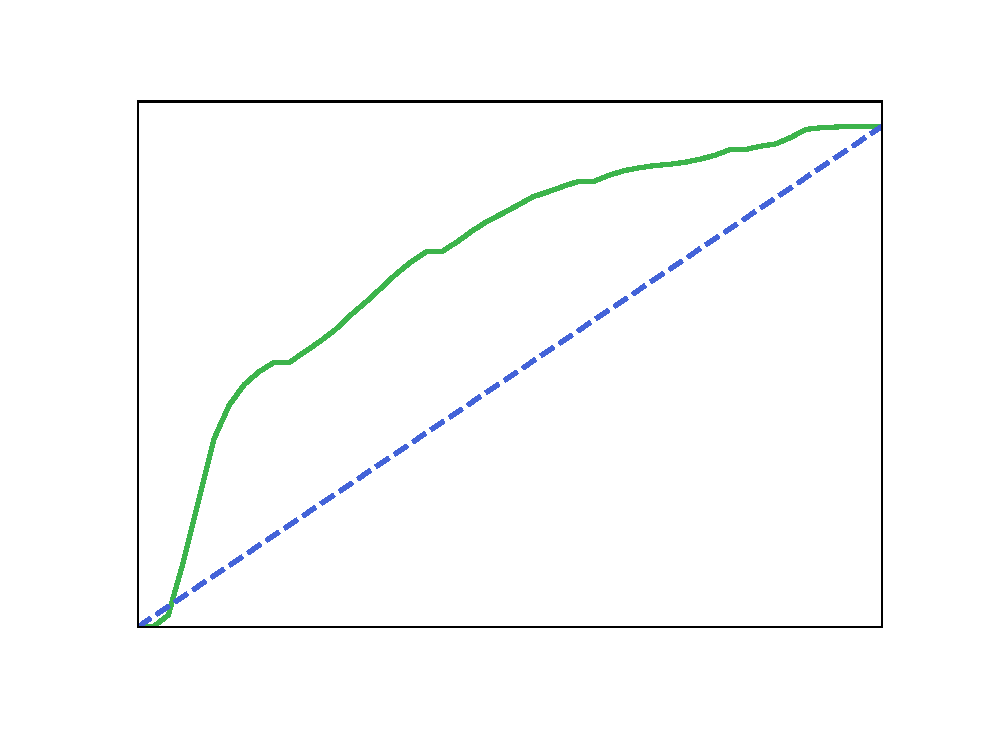
\includegraphics[width=\textwidth,height=.5\textwidth]{Figures/ROC.pgf}

\caption{\Acrlong{ROC} curves of clinical expert and algorithm performance.
For the performance of the algorithm, the \per{95} confidence interval is plotted as well (shaded gray), representing the uncertainty due to randomness in model training}\label{fig:LGG_1p19q_ROC}
\end{figure}


\begin{table}[htbp]
    \sisetup{
        table-number-alignment=center-decimal-marker,
        table-text-alignment = center,
        }
\begin{tabular}{lS[table-format=1.3]S[table-format=1.3]S[table-format=1.3]S[table-format=1.3]S[table-format=1.3]}
    \toprule
    & \textbf{Accuracy}  & \textbf{P-value} & \textbf{AUC} & \textbf{Sensitivity} & \textbf{Specificity}\\
    \midrule
    \textbf{Neurosurgeons}\\
    \hspace{1em}Neurosurgeon 1 & 0.520 & 0.073 & 0.580 & 0.370 & 0.820\\
    \hspace{1em}Neurosurgeon 2 & 0.457 & 0.002 & 0.449 & 0.459 & 0.455\\
    \hspace{1em}Average & 0.489 & {\NA} & 0.515 & 0.415 & 0.638\\
    \\
    \textbf{Neuroradiologists}\\
    \hspace{1em}Neuroradiologist 1 & 0.690 & 0.720 & 0.830 & 0.610 & 0.840\\
    \hspace{1em}Neuroradiologist 2 & 0.574 & 0.266 & 0.792 & 0.459 & 0.795\\
    \hspace{1em}Average& 0.632 & {\NA} & 0.811 & 0.535 & 0.818\\
    \\
    \textbf{Algorithm} & 0.693 & {\NA} & 0.723 & 0.732 & 0.617\\
    \bottomrule

\end{tabular}
\caption{Predictive performance of four clinical experts compared with the algorithm on the \acrshort{TCIA} validation dataset. P-values are determined by a statistical comparison (McNemar) of the accuracy between the clinical experts and the algorithm}\label{tab:LGG_1p19q_clinician_svm_results}
\end{table}


The results of mixing the \cgls{EMC}/\cgls{HMC} dataset and the \cgls{TCIA} dataset are shown in \cref{app:LGG_1p19q_mixing}.
Mixing the datasets leads to a slightly improved performance but still within the \cgls{CI} of the \cgls{EMC}/\cgls{HMC} dataset cross-validation results.

According to the algorithm, the most important features for accurate \acl{1p19qstat} prediction were the cranial/caudal location of the \gls{tumor}, the skewness of the \cgls{T2} \cgls{SI} histogram, and one of the texture features, together with age and sex \cref{fig:LGG_1p19q_feature_importance}.
The algorithm identified a typical \acl{1p19qcodel} glioma as a frontal heterogeneous \gls{tumor} as seen on \cgls{T1C} and \cgls{T2} scans, whereas a typical \acl{1p19qint} glioma was identified as a parietal homogeneous \gls{tumor}, as shown in \cref{fig:LGG_1p19q_Examples}.


\begin{figure}
\centering
\includegraphics[width=\textwidth,height=0.9\textheight]{Figures/Feature_importance.pgf}
\caption{Importance of imaging and demographic features}\label{fig:LGG_1p19q_feature_importance}
\end{figure}


\begin{figure}
     \centering
     \begin{subfigure}[b]{0.8\textwidth}
         \centering
         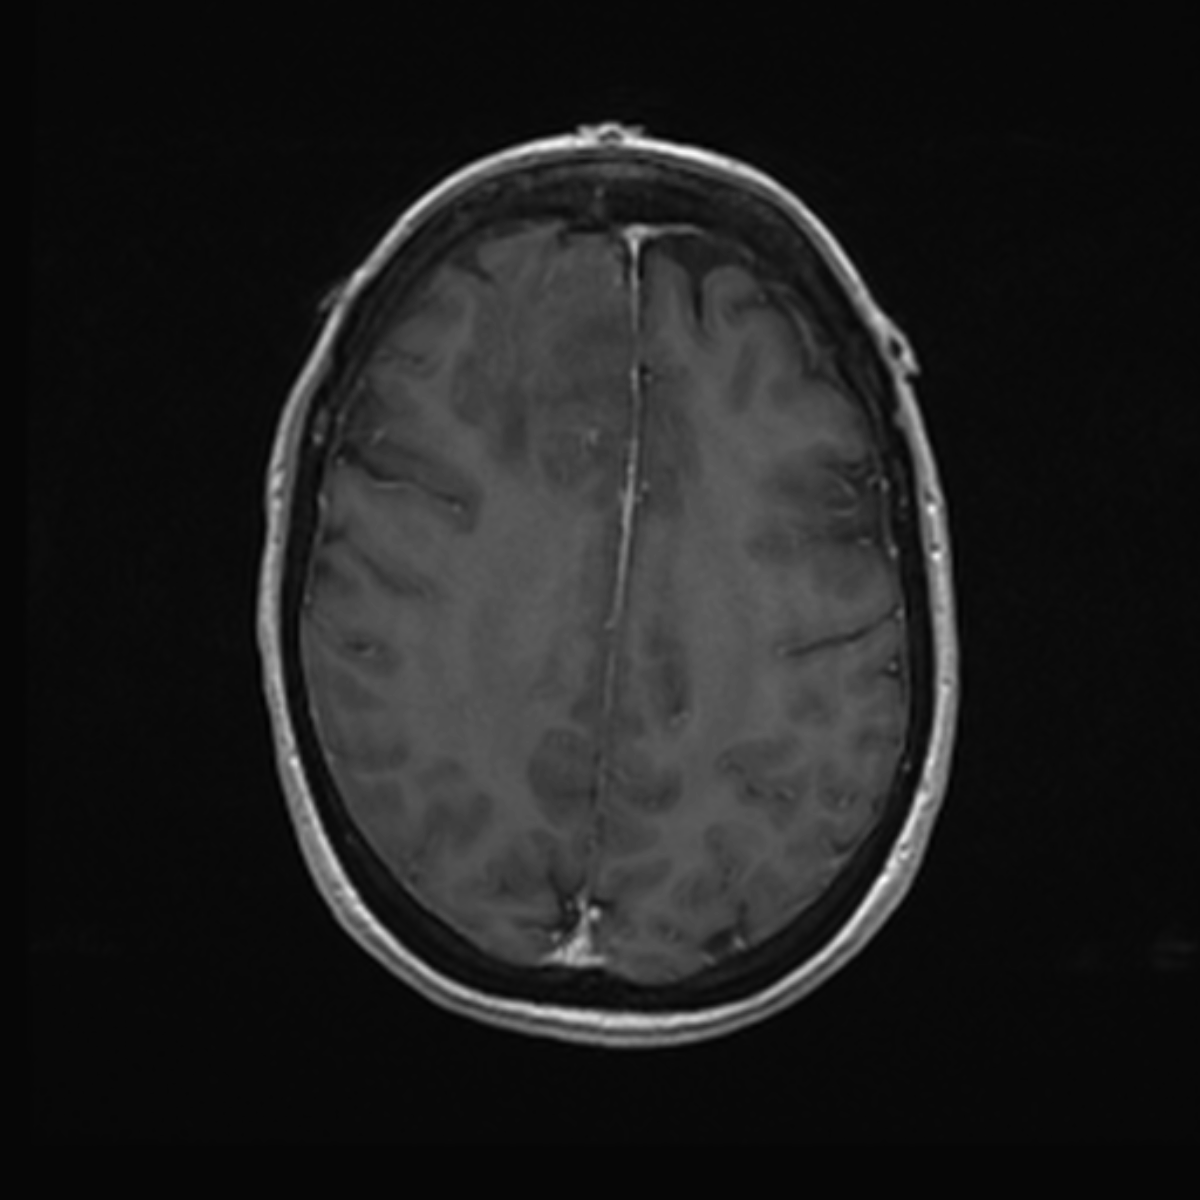
\includegraphics[width=0.475\textwidth]{Figures/LGG_104_codeleted_example_T1.png}
         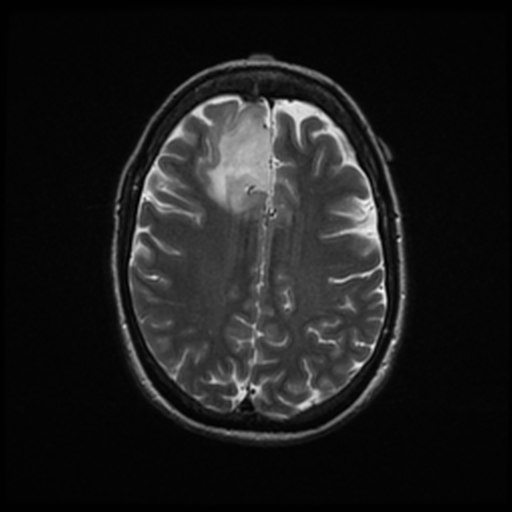
\includegraphics[width=0.475\textwidth]{Figures/LGG_104_codeleted_example_T2.png}
         \caption{A \acl{1p19qcodel} glioma (oligodendroglioma), correctly predicted by the algorithm. The glioma is frontally located, nonenhancing on the \cgls{T1C} \cgls{MR} image, and shows a heterogeneous signal intensity with indistinct border on the \cgls{T2} \cgls{MR} image}\label{fig:LGG_1p19q_example_codeleted}
     \end{subfigure}


     \begin{subfigure}[b]{0.8\textwidth}
         \centering
         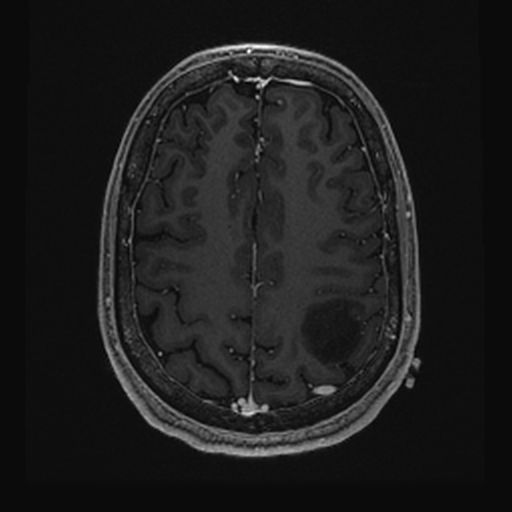
\includegraphics[width=0.475\textwidth]{Figures/LGG_625_intact_example_T1.png}
         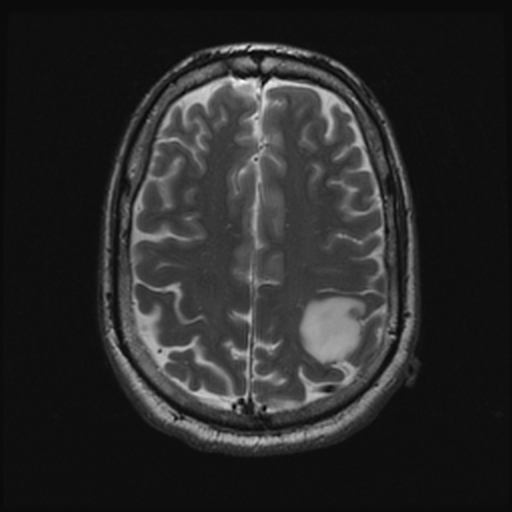
\includegraphics[width=0.475\textwidth]{Figures/LGG_625_intact_example_T2.png}
         \caption{A \acl{1p19qint} glioma (astrocytoma), correctly predicted by the algorithm. The glioma is parietally located, nonenhancing on \cgls{T1C} \cgls{MR} image and shows a homogeneous signal intensity with sharply demarcated border on the \cgls{T2} \cgls{MR} image}\label{fig:LGG_1p19q_example_intact}
     \end{subfigure}

        \caption{\acrshort{T1C} and \acrshort{T2} \acrshort{MR} images of a patient with a \acl{1p19qcodel} glioma (\protect\subref{fig:LGG_1p19q_example_codeleted}) and a patient with a \acl{1p19qint} glioma (\protect\subref{fig:LGG_1p19q_example_intact})}\label{fig:LGG_1p19q_Examples}
\end{figure}



\section{Discussion}

In this study, we developed an algorithm that predicted the \acl{1p19qstat} of presumed \cgls{LGG} noninvasively based on preoperative \cgls{MR} images with an \cgls{AUC} of approximately \num{0.75}.
We tested the algorithm on an external, independent validation dataset.
To the best of our knowledge, this is the first time that this has been done in presumed \cgls{LGG} and thus sets a benchmark for the expected performance in the real-world clinical setting.
The algorithm had a higher \cgls{AUC} than the averaged \cgls{AUC} of the neurosurgeons but lower than the averaged \cgls{AUC} of the neuroradiologists.

To the best of our knowledge, this is the first study performing a radiogenomics-based machine learning study in \cgls{LGG} from the perspective of real-world clinical practice: we included all patients with presumed, non-contrast-enhancing \cgls{LGG}, rather than a selection of patients with histopathologically defined \cgls{LGG}.
This is important, because in a clinical setting the genetic mutation is unknown at first symptomatic presentation.
Because it is known only after surgery and molecular analysis, we aimed to mirror this real-world situation as best as possible by not selecting patients on the basis of histologic \gls{tumor} features but on the imaging features that are available at the time of presentation.
Note that subsequently all lesions were surgically resected to obtain the ground truth data based on confirmed histologic and molecular analysis.
We trained the algorithm on a heterogeneous training dataset and used a separate, completely independent, publicly available dataset with data from an entirely different institute to validate the algorithm.
As such, this study is the first to demonstrate that the performance of a radiogenomics algorithm in predicting the \acl{1p19qstat} of presumed \cgls{LGG} based on \cgls{MR} images was robust and matched expert clinical performance.
Furthermore, we were also able to show which image features were important in the classification, increasing the clinical understanding of the machine learning algorithm and potentially aiding better acceptance, as well as furthering fundamental research into understanding of glioma pathophysiology.

Although other studies did already investigate the noninvasive prediction of the molecular subtype of \cgls{LGG}, these often focused on \cgls{IDH} mutations only and did not consider the \acl{1p19qstat} \autocite{li2017deep, ren2019noninvasive, yu2017noninvasive}.
In comparison with studies that did look at the \acl{1p19qstat}, we used a larger cohort and an external validation dataset \autocite{akkus2017predicting, chang2018deep, han2018non, park2018prediction, shofty2018mri}, which makes our results more robust and generalizable, respectively.
Although one study by \citeauthorref{lu2018machine} did use an independent dataset, this study used only 5 patients to externally validate the \acl{1p19qstat} predictive performance of the algorithm, which severely limits the reliability of its predictive performance.
In addition, that specific study retrospectively selected patients with histopathologically defined \cgls{LGG} only, which represents the diagnosis-treatment workflow in clinical practice less accurately.
The starting point of decision making on the optimal treatment strategy for \cgls{LGG} is the initial diagnosis on first \cgls{MRI}, when a non-contrast-enhancing space occupying lesion is seen, at which point knowledge on the histopathologic grade is not yet available.

The optimal timing and effect of surgical treatment of \cgls{LGG} are extensively being debated within literature and have recently been reevaluated in the light of molecular subclassification after the introduction of \cgls{WHO} 2016 criteria \autocite{wijnenga2017impact, clark2019extent, jakola2017surgical, jiang2017biopsy}.
Currently, the molecular subtype based on \acl{1p19qstat} and \cgls{IDH} mutation can be diagnosed only after obtaining tissue with biopsy or surgery.
Indeed, as our results suggest, it is even for experienced neuro-oncologic surgeons and radiologists a challenge to accurately predict the \acl{1p19qstat} of nonenhancing \glspl{tumor} based on preoperative \cgls{MR} images (\cgls{AUC} of \numrange{0.45}{0.83}).

There are two scenarios in which preoperative, noninvasive prediction of the \acl{1p19qstat} based on \cgls{MRI} would be clinically relevant.
First, some patients are not eligible for surgical resection or diagnostic biopsy due to older age, poor neurologic condition, or \gls{tumor} localization in eloquent brain areas or basal ganglia \autocite{jiang2017biopsy}.
However, knowledge of the molecular \cgls{LGG} subtype might add to a more appropriate (timing of) chemo- and/or radiotherapy regimes (immediate postoperative therapy vs.\ watchful waiting \autocite{ricard2007dynamic}).
Therefore, noninvasive, accurate prediction of the molecular subtype on imaging could help clinicians select the optimal treatment when tissue diagnosis is difficult to obtain.
Second, it is suggested that postsurgical residual \acl{1p19qint}, \cgls{IDH}-mutated \gls{tumor} has a more negative impact on survival than residual \acl{1p19qcodel}, \cgls{IDH}-mutated (oligodendroglioma) \gls{tumor} \autocite{wijnenga2017impact, clark2019extent}.
With presurgical knowledge of the specific molecular subtype, the surgeon can make a better informed decision on whether or not to push the limits of resection at the time of surgery, avoiding on the one hand reresection in case of residual \acl{1p19qint}, \cgls{IDH}-mutated \gls{tumor} and less-justified postsurgical deficits in \acl{1p19qcodel} \gls{tumor} on the other hand.
Clearly, the diagnostic accuracy of our algorithm is as yet too low to rely on for clinical practice.
However, the results are promising because they generalize through multiple datasets, encouraging future research in this direction.

Our study had a few limitations.
First, for this study, only the \cgls{T1C} and \cgls{T2} images were used, whereas diffusion-weighted and perfusion imaging also contain relevant features for the \acl{1p19qstat}.
These sequences were not included in the development of the present algorithm, as these were scarcely available in both datasets.

Second, the \cgls{IDH} mutation status was undetermined in all of the \cgls{TCIA} cases and in 35 cases of the \cgls{EMC}/\cgls{HMC} dataset.
Because molecular subclassification according to the \cgls{WHO} 2016 guidelines is based on both the \acl{1p19qstat} and \cgls{IDH} mutation status, it is important to predict both.
Therefore, for our future work, we are expanding our database with more patients in whom the \gls{tumor} \cgls{IDH} status is known to eventually be able to predict all clinically relevant subtypes of presumed \cgls{LGG}.

There was an imbalance between the \cgls{EMC}/\cgls{HMC} dataset and the \cgls{TCIA} dataset in terms of the number of codeleted and intact cases.
Despite this imbalance, our algorithm still shows similar performance between the cross-validation result of the \cgls{EMC}/\cgls{HMC} dataset and the performance on the \cgls{TCIA} test dataset.

In conclusion, our results suggest that our algorithm can noninvasively predict the \acl{1p19qstat} of presumed \cgls{LGG} with a performance that in general outperforms oncological neurosurgeons.
We evaluated our algorithm on an independent, multicenter dataset, which demonstrated that our algorithm is robust and generalizable.
The prediction of the \acl{1p19qstat} by our algorithm can eventually add value to clinical decision making by tailoring the treatment strategy for patients with presumed \cgls{LGG} even prior to surgery.

\section*{Acknowledgements}

The authors thank the patients who participated in this study and Claudine Nogarede-Bloemendaal for assistance with data collection at the Haaglanden MC\@.
S.R. van der Voort and F. Incekara were funded by the Dutch Cancer Society (KWF project number EMCR 2015-7859).
M.P.A. Starmans and S. Klein were funded by the Netherlands Organisation for Scientific Research (NWO project number 14929-14930).

\begin{subappendices}
\section{Radiogenomics algorithm}\label{app:LGG_1p19q_algorithm}
An in-house radiomics pipeline, \say{PREDICT}, was used for the prediction of the \acl{1p19qstat}\footnote{\url{https://github.com/Svdvoort/PREDICT}}.
This pipeline takes the \cgls{T1C} \cgls{T2} \cgls{MR} images, \gls{tumor} segmentations, and brain segmentations on both scans, and labels indicating \acl{1p19qstat} for each patient which can then be used to train a \cgls{SVM} \autocite{cortes1995support}.
This \cgls{SVM} can then be used to predict the labels for unseen images. In this appendix the different steps of the pipeline are explained.

\subsection{Data pre-processing}
First, the segmentations were transformed to the \cgls{T2} scan and the \cgls{T1C} scans.
If the segmentation was done on \cgls{FLAIR}, the \cgls{FLAIR} scan was registered to the \cgls{T2} scan using SimpleElastix with an affine transform by maximisation of mutual information \autocite{marstal2016simpleelastix}.
The computed transform was used to map the \cgls{FLAIR} segmentation to the \cgls{T2} scan.
Then, the \cgls{T2} scans were registered to the \cgls{T1C} scans.
The computed transformation was used to transform the segmentation from the \cgls{T2} scans to the \cgls{T1C} scan.
This method was applied to both the segmentations originally done on the \cgls{T2} scans, and the ones that were registered to the \cgls{T2} scan from the \cgls{FLAIR}.
All segmentations and registrations were checked by M.S., and manual adjustments of the segmentations were made by F.I. if necessary.

The next step of the pre-processing was to obtain the brain masks, which were created by FSL BET with a setting of 0.5 \autocite{smith2002fast}.
The brain masks were used to normalize the scans.
This was done by extracting the intensity values that lie within the brain mask, after which Z-scoring was applied.
In this way, the mean intensity within the brain mask was 0 and the standard deviation of the intensities within the brain mask 1.
These pre-processed images were then processed by the next step of the algorithm to extract the features.

\subsection{Features}
In total 80 features were used in our algorithm: 78 features from the \cgls{T1C} and the \cgls{T2} images, and age and sex.
These features were split into 5 groups: \gls{tumor} intensity, \gls{tumor} texture, \gls{tumor} shape, \gls{tumor} location, and demographic features.
All of these features were only extracted within the \gls{tumor} mask.

Image intensity was described using 11 features: minimum, maximum, mean, median, standard deviation, skewness, kurtosis, range from the 2nd to 98th percentile, range from the 25th to 75th percentile (the quartile range), the mode position (the bin in the intensity histogram which had the highest occurrence) of the intensity and the energy (defined as: $E = \sum \left( {\left( I + \min(I)\right)}^2\right)$, where $I$ is the image intensity).
These features were calculated over the entire \gls{tumor} in 3D.

Rotation invariant \cglspl{LBP} were used to describe the texture of the \gls{tumor} \autocite{ojala2002multiresolution}.
The advantage of \cglspl{LBP} is that they are grayscale invariant, meaning that not the intensity values themselves, but the differences between intensity values of different voxels are taken into account.
This is an advantage when using \cgls{MRI} scans, because in weighted \cgls{MRI} scans the absolute values signal intensities themselves do not carry information, it is only the difference in gray values in the image.
\cgls{LBP} features were determined for a radius of 1, 3 and 5 with 8, 24 and 24 points, respectively.
The \cgls{LBP} was determined for each slice of the \cgls{MRI} scan in which \gls{tumor} was present.
The results over all pixels within the \gls{tumor} and slices containing \gls{tumor} were then concatenated and consequently the mean, standard deviation, median, kurtosis and skewness, and peak value were calculated for each setting, resulting in 18 \cgls{LBP} features.

The intensity features and the texture features were calculated on both the \cgls{T1C} and \cgls{T2} scan, resulting in 58 features.

Shape features were derived from the segmentation on the \cgls{T2} image.
Shape features consisted of the compactness, radial distance, roughness, convexity, circular variance (cvar), ratio of principal axes (prax), elliptical variance (evar) and solidity \autocite{peura1997efficiency, xu2012comprehensive}.
All of these features were calculated on a per-slice basis (only for slices that contained \gls{tumor}), after which the mean and standard deviation of the features over the slices were included as features in the algorithm, resulting in 16 features.
The volume was also taking as a 3D shape feature, resulting in 17 shape features.

\Gls{tumor} location was determined by using the \cgls{COM} from the brain mask and \cgls{COM} of the \gls{tumor} segmentation.
The anterior/posterior, left/right and inferior/superior coordinate of the vector pointing from the \cgls{COM} of the brain to the \cgls{COM} of the \gls{tumor} were then included as features, resulting in 3 location features.

Patient age and patient sex were included as the demographic features.
An overview of all the features is given in \cref{tab:LGG_1p19q_ISBI}, along with the \cgls{IBSI} code when the feature matched with one included in the \cgls{IBSI} \autocite{zwanenburg2016image}.
Many of our features are based on local binary patterns, which are currently considered outside the scope of \cgls{IBSI}.
However, preliminary experiments have indicated that including these features improves the performance of the classifier (results not shown).

Z-scoring was applied to the features (normalized such that the mean of the features was 0 and the standard deviation was 1).
This was done based only on the training set; the resulting normalisation settings were saved to apply the same normalisation to the validation set.

\begin{table}[htbp]
    \footnotesize
    \begin{tabular}{L{3.9cm}R{0.3cm}L{5.7cm}}
        \toprule
        \multicolumn{2}{r}{\textbf{Number of features}}&\textbf{\acrshort{IBSI} code}\\
        \midrule
        \textbf{Demographics} & 2 &  \\
        \hspace{1em}Age & 1 & \NA \\
        \hspace{1em}Sex & 1 & \NA \\
        \addlinespace
        \textbf{Location features} & 3 &  \\
        \multicolumn{3}{l}{\textit{Derived from \gls{tumor} segmentation and brain mask}}\\
        \hspace{1em}Anterior/Posterior position & 1 & None \\
        \hspace{1em}Left/Right position & 1 & None \\
        \hspace{1em}Inferior/Superior Position & 1 & None \\
        \addlinespace
        \textbf{Shape features} & 17 &  \\
        \multicolumn{3}{l}{\textit{Derived from \gls{tumor} segmentation}}  \\
        \multicolumn{3}{l}{\textit{Average and standard deviation over all slices are determined}}\\
        \multicolumn{3}{l}{\textit{for all features (except for volume)}}\\
        \hspace{1em}Compactness & 2 & KRCK \\
        \hspace{1em}Convexity & 2 & None \\
        \hspace{1em}Circular variance & 2 & None \\
        \hspace{1em}Elliptic variance & 2 & None \\
        \hspace{1em}Ratio of principal axis & 2 & None \\
        \hspace{1em}Radial distance & 2 & None \\
        \hspace{1em}Roughness & 2 & None \\
        \hspace{1em}Solidity & 2 & Inverse of 7T7F \\
        \hspace{1em}Volume & 1 & 2PR5 \\
        \addlinespace
        \textbf{Intensity features} & 22 &  \\
        \multicolumn{3}{l}{\textit{Derived from \gls{T1C} and \gls{T2} scans}}  \\
        \hspace{1em}Energy & 2 & N8CA, with minimum intensity added \\
        \hspace{1em}Kurtosis & 2 & IPH6 \\
        \hspace{1em}Max & 2 & 84IY \\
        \hspace{1em}Mean & 2 & Q4LE \\
        \hspace{1em}Median & 2 & Y12H \\
        \hspace{1em}Min & 2 & 1GSF \\
        \hspace{1em}Peak & 2 & None \\
        \hspace{1em}Range & 2 & 20JQ, but based on \nth{2} and \nth{98} percentile \\
        \hspace{1em}Skewness & 2 & KE2A \\
        \hspace{1em}Standard deviation & 2 & Square root of ECT3 \\
        \hspace{1em}Quartile range & 2 & SALO \\
        \addlinespace
        \textbf{Texture features} & 36 &  \\
        \multicolumn{3}{l}{\textit{Derived from \gls{T1C} and \gls{T2} scans}} \\
        \multicolumn{3}{l}{\textit{Kurtosis, mean, median, peak, skewness, and standard deviation are determined}}\\
        \multicolumn{3}{l}{\textit{for each \acrshort{LBP} setting}}\\
        \hspace{1em}\acrshort{LBP} R1P8 & 12 & None \\
        \hspace{1em}\acrshort{LBP} R3P24 & 12 & None \\
        \hspace{1em}\acrshort{LBP} R5P24 & 12 & None \\
        \addlinespace
        \textbf{Total} & 80 & \\
        \bottomrule
    \end{tabular}
    \caption{Overview of the features included in the algorithm. The \acrshort{IBSI} column indicates the code of the feature if it is present in the \acrshort{IBSI}. \acrshort{LBP} RxPy indicated a \acrshort{LBP} with a radius of x and y points. Abbreviations: \acrcaption{IBSI}, \acrcaption{LBP}}\label{tab:LGG_1p19q_ISBI}
\end{table}

\subsection{Over-sampling of the minority class}
There was an imbalance in the training dataset as there were more examples of \acl{1p19qint} than of \acl{1p19qcodel} \glspl{tumor}.
As a result, it was more difficult for the algorithm to correctly predict \acl{1p19qcodel} \glspl{tumor} within the training dataset.
To (partially) solve this problem we used \cgls{SMOTE}.
\cgls{SMOTE} allows for the oversampling of the minority class and synthetically increased the number of samples for the \acl{1p19qcodel} class \autocite{chawla2002smote}.
Here, an \cgls{SVM} with a polynomial kernel was used to create the synthetic examples, with a ratio of 1 (meaning that there will be an equal number of samples from both classes) using 5 neighbours.

\subsection{Classification}
\cglspl{SVM} were used as classification algorithm \autocite{cortes1995support}.
\cglspl{SVM} were constructed using scikit-learn with a polynomial kernel \autocite{pedregosa2011scikit}.
The polynomial kernel was defined as:
\begin{equation*}
    K(X, Y) = {\left(\gamma \langle X, Y \rangle + C_0\right)}^P
\end{equation*}
\cgls{SVM} were constructed with a maximum of \num{1e7} iterations.
The hyperparameters of the \cgls{SVM} were optimized using a 5-fold cross-validation where \per{20} of the training dataset was used as an internal validation set.
A random search of \num{50000} iterations was used to find the optimal hyperparameters.
This optimization search for the optimal $C$, the regularization parameter of the \cgls{SVM}, as well as three parameters of the polynomial kernel: $\gamma$, which defines how much each sample is weighted, $C_0$, a trade-off between high-order and low-order terms, and $P$, the order of the polynomial kernel.

The distributions for the parameters are presented in \cref{tab:LGG_1p19q_svm_parameters}.

\begin{table}[htbp]
\centering
\begin{tabular}{L{2cm} C{2.5cm} C{2.5cm}}
    \toprule
    \textbf{Parameter} & \textbf{Lower bound} & \textbf{Upper bound} \\
    \midrule
    $C$ & 0 & \num{1e6}\\
    $P$ & 1 & 7\\
    $C_0$ & 0 & \num{1e3}\\
    $\gamma$ & \num{1e-5} & 1\\
    \bottomrule
\end{tabular}
\caption{Overview of the range of hyperparameters used in the optimization of the \acrshort{SVM}}\label{tab:LGG_1p19q_svm_parameters}
\end{table}


The optimal hyperparameters were chosen based on the settings that gave the highest average area under curve over the 5 folds.
Using these optimal hyperparameters, the final \cgls{SVM} was then constructed using the complete training dataset.

\subsection{Ensemble \acrshort{SVM}}
To increase the predictive performance and minimize the variability of the predictions, an ensemble of \cglspl{SVM} was constructed.
Five trained \cglspl{SVM} were taken to form the ensemble.
All 5 \cglspl{SVM} were then used to predict a test sample.
The posteriors of the \cglspl{SVM} were averaged for the sample.
Based on this averaged posterior the final label was determined (positive class if posterior \num{>= 0.5} and negative class if posterior \num{< 0.5}).
To form the 100 ensembles 500 \cglspl{SVM} had to be trained.
No single \cgls{SVM} was used in two different ensembles: all ensembles were completely unique.
The resulting 100 ensemble \cglspl{SVM} could then be used to make a prediction of the \acl{1p19qstat} for a new sample.

\clearpage
\section{Excluded patients from TCIA-LGG dataset}\label{app:LGG_1p19q_exclusion}

\begin{table}[h]
    \centering
    \begin{tabular}{ll}
        \toprule
        \textbf{Patient ID} & \textbf{Reason for Exclusion} \\
        \midrule
        LGG-223 & Enhancement \\
        LGG-234 & Enhancement \\
        LGG-241 & Enhancement \\
        LGG-254 & Post-biopsy \\
        LGG-260 & Enhancement \\
        LGG-282 & Enhancement \\
        LGG-295 & Enhancement \\
        LGG-296 & Post-biopsy \\
        LGG-307 & Enhancement \\
        LGG-310 & Post-biopsy \\
        LGG-313 & Post-biopsy \\
        LGG-334 & Post-biopsy \\
        LGG-338 & Enhancement \\
        LGG-354 & Enhancement \\
        LGG-365 & Enhancement \\
        LGG-367 & Post-biopsy \\
        LGG-377 & Enhancement \\
        LGG-387 & Enhancement \\
        LGG-500 & Age \textless 18 years \\
        LGG-506 & Enhancement \\
        LGG-532 & Age \textless 18 years \\
        LGG-545 & No \gls{T1C} image \\
        LGG-558 & No \gls{T1C} image \\
        LGG-561 & Enhancement \\
        LGG-563 & No \gls{T1C} image \\
        LGG-594 & Enhancement \\
        LGG-600 & Enhancement \\
        LGG-601 & Post-biopsy \\
        LGG-634 & Enhancement \\
        LGG-642 & Enhancement\\
        \bottomrule
    \end{tabular}
    \caption{Overview of patients excluded from the TCIA-LGG dataset}
\end{table}

\clearpage

\section{Results of mixing \glsfmtshort{EMC}/\glsfmtshort{HMC} and \glsfmtshort{TCIA} datasets}\label{app:LGG_1p19q_mixing}

We evaluated the effect of mixing the \cgls{EMC}/\cgls{HMC} and \cgls{TCIA} datasets, instead of using them as separate training and validation set.
This was done using the same cross-validation approach as was used for the \cgls{EMC}/\cgls{HMC} dataset cross-validation.
In this case all 413 patients were pooled together.
Then 100 iterations of stratified random-split cross-validation with \per{80} of the dataset used for training and \per{20} of the dataset used for validation was performed.
The results are shown in \cref{tab:LGG_1p19q_mixed_results}.

\begin{table}[h]
\centering
\sisetup{
    table-number-alignment = center,
    table-text-alignment = center,
    }
\begin{tabular}{L{2cm} S[table-format=1.3] S[table-format=2.7] S[table-format=1.3]  S[table-format=2.7]}
% \begin{tabular}{L{2cm} C{4cm} C{4cm}}
    \toprule
    & \multicolumn{2}{c}{\thead{Combined \acrshort{EMC}/\acrshort{HMC}\\and \acrshort{TCIA} dataset\\(N=413)}} & \multicolumn{2}{c}{\thead{\acrshort{EMC}/\acrshort{HMC} dataset\\(N=284)}} \\
    \cmidrule(lr){2-3} \cmidrule(lr){4-5}
    & {Mean} & {\SI{95}{\percent} CI} & {Mean} & {\SI{95}{\percent} CI}\\
    \midrule
    Accuracy &  0.717 & \numrange{0.670}{0.764} & 0.698 & \numrange{0.636}{0.706}\\
    \acrshort{AUC} & 0.780 & \numrange{0.729}{0.830} & 0.755 & \numrange{0.694}{0.817}\\
    F1-score & 0.717 & \numrange{0.670}{0.763} & 0.701 & \numrange{0.640}{0.761}\\
    Precision & 0.676 & \numrange{0.620}{0.732} & 0.570 & \numrange{0.491}{0.649}\\
    Sensitivity & 0.710 & \numrange{0.637}{0.783} & 0.657 & \numrange{0.562}{0.752}\\
    Specificity & 0.723 & \numrange{0.658}{0.788} & 0.721 & \numrange{0.628}{0.813}\\
    \bottomrule
\end{tabular}
\caption{Cross-validation results of mixing the \acrshort{EMC}/\acrshort{HMC} dataset with the \acrshort{TCIA} dataset. The results of the cross-validation on only the \acrshort{EMC}/\acrshort{HMC} dataset are also shown. Abbreviations: \acrcaption{CI}}\label{tab:LGG_1p19q_mixed_results}
\end{table}

The results for the combined \cgls{EMC}/\cgls{HMC} and \cgls{TCIA} dataset show a slight improvement over the cross-validation on the \cgls{EMC}/\cgls{HMC} dataset alone but they are still within the confidence interval of the \cgls{EMC}/\cgls{HMC} dataset results, except for the precision.
This shows that although there is a slight improvement, our algorithm is already quite robust and adding more data (from a different source) does not lead to a large increase in performance.


\end{subappendices}
